\documentclass[french]{article}
\usepackage{graphicx}
\usepackage{caption}
\usepackage[T1]{fontenc}
\usepackage[utf8]{inputenc}
\usepackage{lmodern}
\usepackage[a4paper]{geometry}
\usepackage{babel}
\usepackage[unicode=true,pdfusetitle,bookmarks=true,bookmarksnumbered=false,bookmarksopen=false,
breaklinks=false,pdfborder={0 0 0},backref=false,colorlinks=true]{hyperref}

\author{Andrea Brugnoli \\ 
\hspace{2.8pt} Docteur ISAE-Supaéro 2020\\
Ingénieur ISAE-Supaéro 2017}
\title{Méthodes numériques pour la révolution digitale des jumeaux numériques: de la modélisation multi-physique haute fidélité aux modèles réduits pour la prise de décision}

\date{}

\begin{document}

\maketitle

\large{Dossier de candidature au prix de la fondation Jean-Jacques et Félicia
	Lopez-Loreta pour l’excellence académique}


\begin{figure}[h]
	\centering
	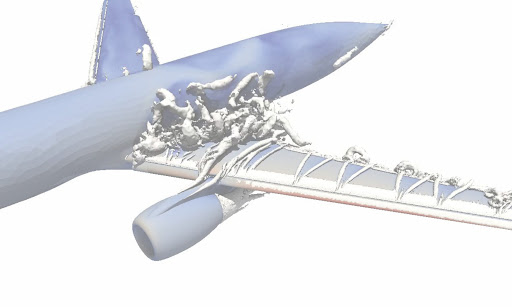
\includegraphics[width=.95\textwidth]{3Dplane.jpg}
	\captionsetup{labelformat=empty}
	\caption{Source: \href{http://www.fenics-hpc.org/}{FEniCS-HPC website}}
\end{figure}





\thispagestyle{empty}

\newpage

\section{Contexte et Objectifs du projet}

\subsection{Le candidat}
La technologie et les sciences et leur impacte sur l'humaine m'ont toujours intéressé. C'est pour cela que j'ai opté pour un baccalauréat littéraire avec option informatique (100/100 obtenu en 2011 a Vérone, Italie). Après mon baccalauréat\footnote{En Italie il est possible d'accéder aux universités scientifique après un Bac. L.}, j'ai obtenu une licence en ingénierie mécanique du Politecnico de Milan (110/100 summa cum laude). Pendant la première année du master en ingénierie Spatiale, j'ai décide de partir a'l'étranger et j'ai choisi d'effectuer un double diplôme a l'ISAE. J'ai pu approfondir mes connaissances en automatique grâce a un master recherche en collaboration avec Supélec/Université Paris Saclay, ainsi que mes compétences en mathématiques appliquées grâce au domaine SXS (Systèmes compleXes et Simulation). Mon intérêt pour les systèmes dynamiques et la simulation numérique m'a amener au CNES pour mon stage de fin études. 



\subsection{Contexte}

\subsection{Le projet}

\section{Organisation du projet et mise en œuvre}

\subsection{Partenariats académiques et retombées industrielles}

\subsection{Le plan}

\subsection{Budjet}




\bibliographystyle{unsrt}
\nocite*
\bibliography{biblio_articles}

\end{document}
